\documentclass[a4paper,9pt]{extarticle}

\title{cheat sheet}
\date{2017-09-16}

\usepackage{pew}

\begin{document}
\begin{multicols*}{2}
\section{Introduction}
\subsection{Events [2.2]}
\begin{enumerate}[label=\bfseries (\arabic*)] \itemsep0pt \parskip0pt
    \item The result $u_1$ of a random trial is called \textbf{outcome}.
    \item The set of all possible outcomes is called \textbf{sample space $\Omega$}.
    \item A collection of outcomes $A$ is called \textbf{event}.
\end{enumerate}

Thus an event is a subset of the sample space (or possibly the whole sample space).

The events $A_1, ..., A_n$ are said to be \textbf{mutually exclusive} (or \textbf{mutually disjoint}) if all pairs $A_i, A_j$ are exclusive; that is, if it is impossible that two or more of these events take place at the same time.

\subsection{Sample spaces [2.2]}
If the number of outcomes is finite or denumerably infinite, $\Omega$ is said to be a \textbf{discrete sample space}. More particularly, if the number is finite, $\Omega$ is said to be a \textbf{finite sample space}.

If the number of outcomes is neither finite nor denumerably infinite, $\Omega$ is said to be a \textbf{continuous sample space}.

\subsection{Kolmogorov's System of Axioms [2.3]}
The following axioms for the probabilities $P(\cdot)$ should be fulfilled:
\begin{enumerate}[label=\bfseries A\arabic*.] \itemsep0pt \parskip0pt
    \item If $A$ is any event, then $0 \leq P(A) \leq 1$.
    \item If $\Omega$ is the entire sample space, then $P(\Omega) = 1$.
    \item ("Addition Formula"). If $A$ and $B$ are mutually exclusive events, then $P(A \cup B) = P(A) + P(B)$.
\end{enumerate}

The sample space $\Omega$ and the probabilities $P(\cdot)$ together constitute a \textbf{probability space}.

\subsection{Results from Kolmogorov's system [2.3]}
\textbf{Complement Theorem}
\begin{equation}
    P(A*) = 1 - P(A)
\end{equation}
\begin{equation}
    P(\varnothing) = 0
\end{equation}

\noindent \textbf{Addition Theorem}
\begin{equation}
    \begin{split}
        P(A \cup B) & = P(A) + P(B) + P(A \cap B) \\
        P(A \cup B \cup C) & = P(A) + P(B) + P(C) - P(A \cap B) \\
        & - P(A \cap C) - P(B \cap C) + P(A \cap B \cap C)
    \end{split}
\end{equation}

\noindent \textbf{Boole's Inequality}
\begin{equation}
    \begin{split}
        P(A \cup B) & \leq P(A) + P(B) \\
        P(A \cup B \cup C) & \leq P(A) + P(B \cup C) \\
        & \leq P(A) + P(B) + P(C)
    \end{split}
\end{equation}

\subsection{Probabilities in Discrete Sample Spaces [2.4]}
\begin{equation} \label{2.4.1}
    P(u_i) = 1/m \quad (i = 1, 2, \ldots, m)
\end{equation}
If (\ref{2.4.1}), we have a \textbf{uniform probability distribution}. \\

An event $A$ with $g$ outcomes, has \textbf{$g$ favourable cases}. That means there are \textbf{$m$ possible cases} in $\Omega$. We then determine $P(A)$ from the addition formula by adding the probabilities $m$ of the $g$ outcomes. Hence,
\begin{equation}
    P(A) = g/m
\end{equation}

\subsection{Urn model [2.4]}
Let's examine the probability of drawing exactly $k$ white balls from an urn containing $a$ white and $b$ black balls, $n$ balls are drawn.

If one ball at a time is drawn at random without returning it to the urn, the drawings are said to be made \textbf{without replacement}. The probability is then:
\begin{equation}
    \frac{\binom{a}{k} \binom{b}{n-k}}{\binom{a + b}{n}}
\end{equation}

If one ball at a time is drawn at random and is returned before the next ball is drawn, the drawings are said to be made \textbf{with replacement}. The probability is then:
\begin{equation}
    \binom{n}{k} p^k q^{n-k}
\end{equation}
where
\begin{equation}
    p = \frac{a}{a+b}, \quad q = 1 - p = \frac{b}{a+b}
\end{equation}

\subsection{Conditional Probability [2.5]}
\begin{equation}
    \begin{split}
        P(B|A) & = \frac{P(A \cap B)}{P(A)} \\
        P(A \cap B) & = P(A) P(B|A) = P(B) P(A|B)
    \end{split}
\end{equation}

is called the \textbf{conditional probability of B given A}.
{\centering 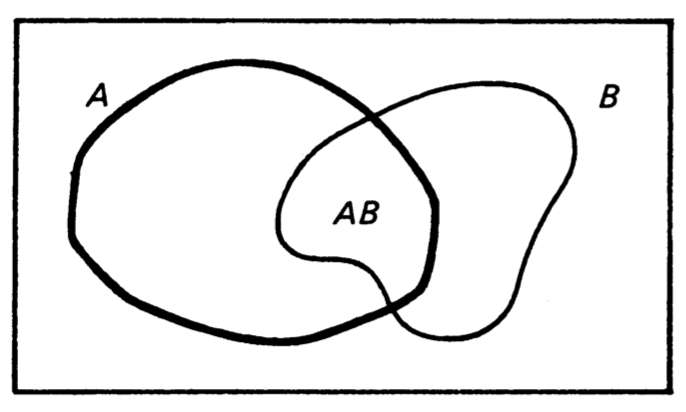
\includegraphics[scale=0.25]{conditional-probability} \par}

From this we can derive the \textbf{Total Probability Theorem}. If the events $H_1, H_2, \dots , H_n$ are mutually exclusive, have positive probabilities, and together fill $\Omega$ completely, any event $A$ satisfies the formula:
\begin{equation}
    P(A) = \sum_{i=1}^n P(H_i) P(A|H_i)
\end{equation}
{\centering 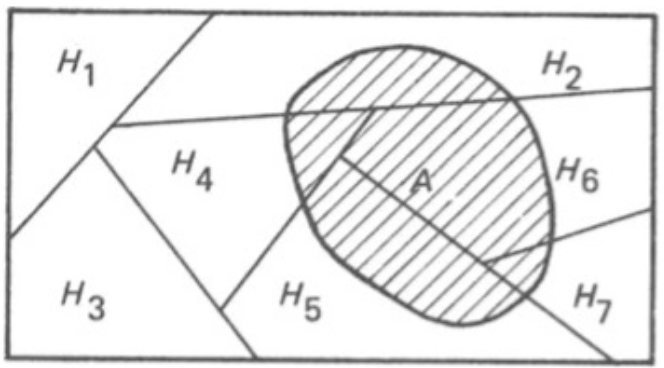
\includegraphics[scale=0.25]{total-probability} \par}

And \textbf{Bayes' Theorem}:
\begin{equation}
    P(H_i|A) = \frac{P(H_i) P(A|H_i)}{\sum_{j=1}^n P(H_j) P(A|H_j)}
\end{equation}

\subsection{Independent Events [2.6]}
\begin{equation} \label{2.6.1}
    P(A \cap B) = P(A) P(B),
\end{equation}
If (\ref{2.6.1}), then $A$ and $B$ are said to be \textbf{independent events}. This can be extended to three events. Consequence:

If the events $A_1, A_2, \dots, A_n$ are independent and $P(A_i)=p_i$, then the probability that at least one of them occurs is equal to
\begin{equation}
    1 - (1 - p_1)(1 - p_2) \cdots (1 - p_n)
\end{equation}

If the events $A_i$ are independent and each one of them occurs with probability $p$, then the probability that at least one of them occurs is equal to $1 - (1 - p)^n$.

Two trials as \textbf{independent}, if the result of one does not affect, or is not affected by, the result of the other. An important special case is provided by \textbf{repeated trials}.

\subsection{Theorems in Combinatorics [2.7]}
Drawing $n$ elements from $N$:

\renewcommand{\arraystretch}{1.5}
\begin{tabulary}{1.0\textwidth}{r|c|c}
    & with replacement & without replacement \\ \hline
    order & $N^n$ & $N (N-1) \cdots (N-n+1)$ \\ \hline
    no order & $\binom{N+n-1}{n}$ & $\binom{N}{n}$ \\
\end{tabulary}

\rule{0pt}{0.5em}
\renewcommand{\arraystretch}{1}

The \textbf{multiplication principle} states: If choice 1 can be performed in $a_1$ ways and choice 2 in $a_2$ ways, then there are $a_1 a_2$ ways to perform both choices. In the case of three choices, the number of ways is $a_1 a_2 a_3$, and so on.

\section{One-Dimensional Random Variables}
\subsection{General Description of Random Variables [3.2]}
A random variable ($rv$) is a function defined on a sample space.

\subsection{Distribution Function [3.3]}
For a given real number $x$ we compute the probability $P(X \leq x)$, such that $X$ is smaller than or equal to $x$. This procedure is performed for any $x$. We then obtain a function $F_X(x) = P(X  \leq x)$ defined for all $x$ in the interval $-\infty < x < \infty$.

$F_X(x) = P(X  \leq x)$ is called the (cumulative) distribution function of the $rv$ $X$.

{\centering 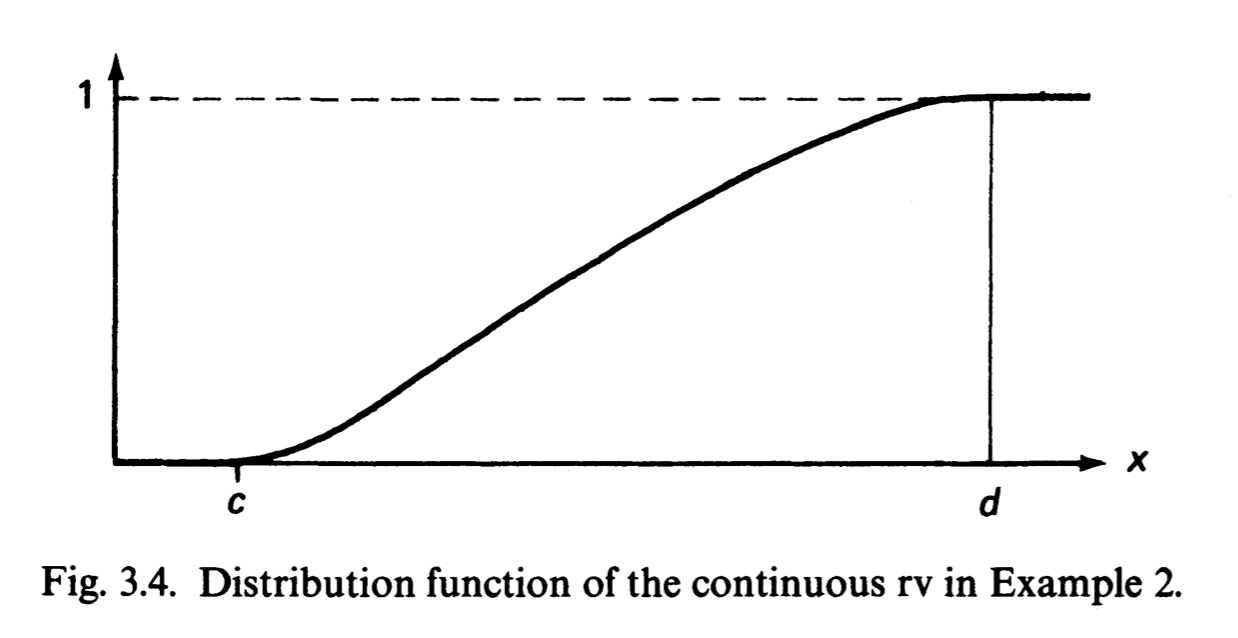
\includegraphics[scale=0.25]{distribution-function} \par}

\textbf{Theorem 1.} The distribution function $F_X(x)$ of a $rv$ $X$ has the properties:
\begin{equation} \label{3.2.1}
    F_X(x) \rightarrow \begin{cases}
        0 \\
        1
    \end{cases} when \quad x \rightarrow \begin{cases}
        -\infty \\
        \infty
    \end{cases}
\end{equation}

\begin{equation} \label{3.2.2}
    F_X(x) \quad \text{is a nondecreasing function of} \quad x;
\end{equation}

\begin{equation} \label{3.2.3}
    F_X(x) \quad \text{is continuous from the right for any} \quad x
\end{equation}

\textbf{Theorem 2.} If $a \leq b$, then
\begin{equation} \label{3.2.3}
    F_X(b) - F_X(a) = P(a < X \leq b)
\end{equation}

\end{multicols*}
\end{document}
